\chapter{Propulsion}
\label{ch:Propulsion}
In this chapter, the procedure to size the propulsion subsystem of the \textit{Swing} will be presented, discussed, motivated and performed.
The design procedure of the propulsion subsystem is summarised and shown in the flowchart of \Cref{fig:propsizingflowchart}.
Insights on the correlation between key requirements and design variables are instead found in \Cref{fig:n2prop}.
After a brief introduction to the concept of disc loading,
following directly from the structure proposed in \Cref{fig:propsizingflowchart}, \Cref{sec:enginesconfigchoice}
will determine the ideal number of engines and their placement along the wing.
To follow is the design of the propellers in \Cref{sec:propdesign} and the choice of suitable OTS engines in \Cref{sec:engineschoice}.
The chapter is concluded by \Cref{sec:propulsionVandV} in which the numerical models used are verified and validated.

\begin{figure}[H]
    \centering
    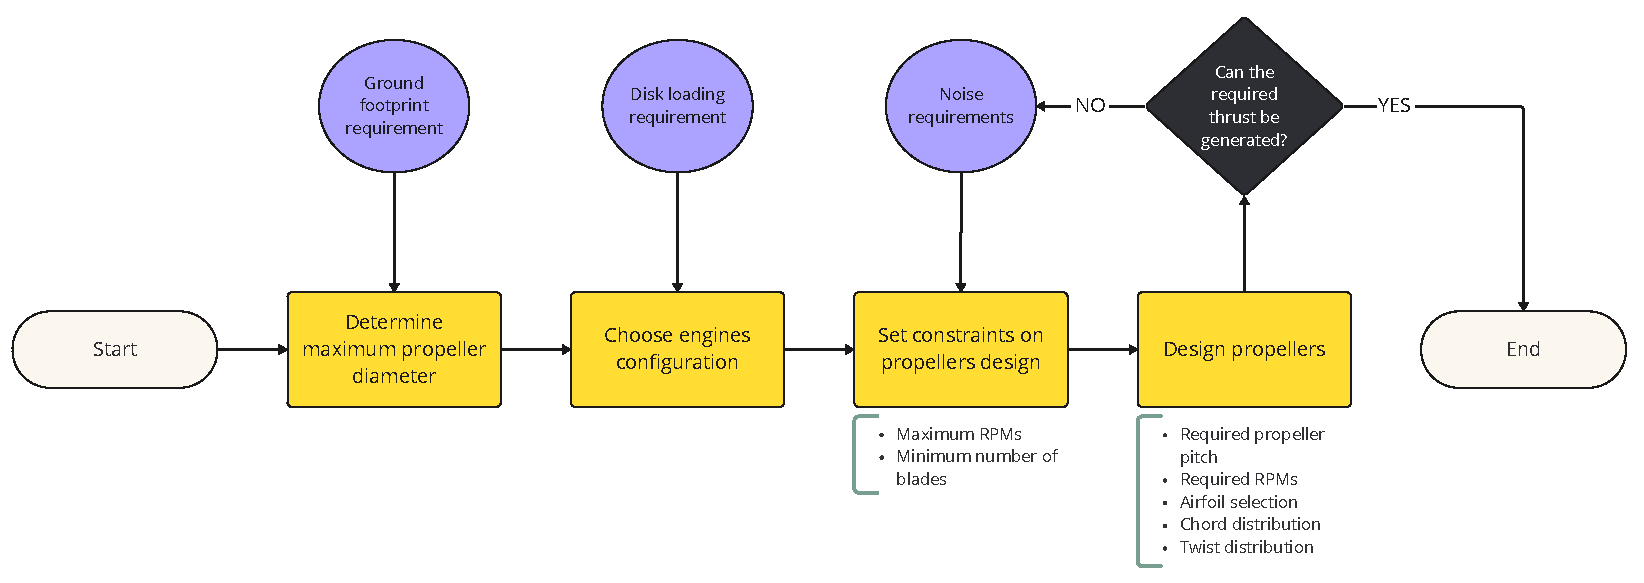
\includegraphics[width=\linewidth]{figures/Propulsion/propflowchart}
    \caption{Flowchart of the propulsion sizing procedure.}
    \label{fig:propsizingflowchart}
\end{figure}
\begin{figure}[H]
    \centering
    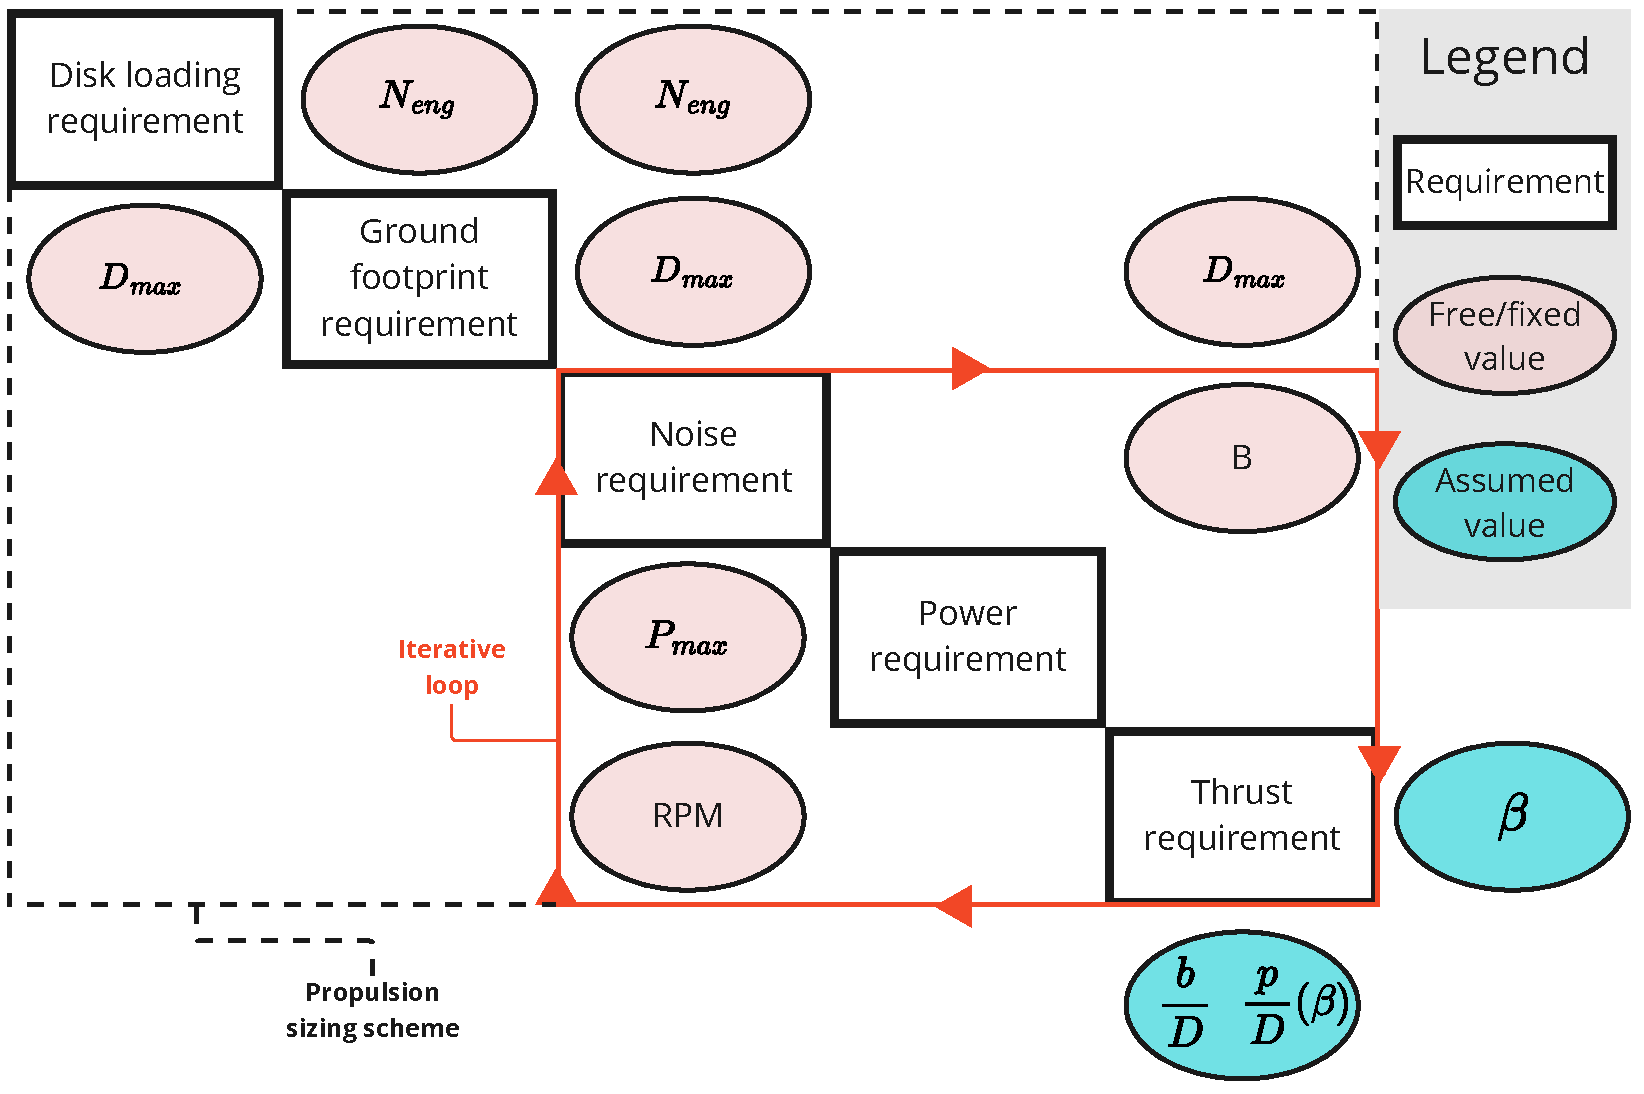
\includegraphics[width=0.9\linewidth]{figures/Propulsion/propN2}
    \caption{N2 chart for propulsion sizing.}
    \label{fig:n2prop}
\end{figure}

\subsubsection{Disc Loading}
Being of crucial importance, the concept of disc loading is here preemptively introduced, and will be used extensively in the sections to follow.
The disc loading is a parameter that influences the performance in many ways, accounting for the average change of pressure over the rotor disc; it can thus be seen as an indication of how heavily each rotor is loaded.
Its maximum (limiting) value can be computed as indicated in \Cref{eq:disc_loading}:
\begin{equation}
    \label{eq:disc_loading}
    \mathrm{DL} = \cfrac{T_{\max}}{S_{\text{disc}} \cdot g \cdot N_{\text{eng}}}
\end{equation}
$\mathrm{DL}$ being the disc loading in \unit{kg/m^2}, $T_{\max}$ the maximum thrust experienced over the mission span, $S_{\text{disc}}$ the area of one rotor, $g$ the gravitational acceleration, and $N_{\text{eng}}$ the number of engines contributing to producing the total thrust.
Here $T_{\max}$ is taken to be $2\cdot W_\text{MTOW}$, in agreement with the maximum thrust requirement (CO-3-STK03-3).
Since the general requirement for multicopters, which accounts for the \textit{Swing} in VTOL configuration, is that the rotors should create twice the thrust required to hover \cite{goli2023experimental}, the design thrust-to-weight ratio ought to be 2 (requirement CO-3-STK03-3).


% \begin{minipage}{.45\linewidth}
%     \begin{equation}
%         \label{eq:hov_eff}
%         \cfrac{w_{0}}{P} = \cfrac{w_{0} \cdot \sqrt{2 \cdot \rho \cdot S_{\text{disc}}}}{(T)^{3/2}} \cdot M
%     \end{equation}
% \end{minipage}


\section{Engines Configuration}
\label{sec:enginesconfigchoice}
% how many engines, engines placement, 
Before delving deeper into propulsion sizing, the ideal number of engines, $N_{\text{eng}}$, must first be determined (engines configuration) as it forms the baseline for any type of propulsion calculations and assessments.
The choice was ultimately based on considerations regarding disc loading and safety, as discussed below, leading to the trade-off of \Cref{tab:tradeoff}.

\subsection{Disc Loading Analysis and Discussion}
\label{subsec:discloadanalysis}
Only configurations comprising of four, six, eight, and ten total rotors are considered, as less than four engines would unacceptably hinder vehicle controllability \cite{du2015controllability} while having more than ten would not allow meeting the requirement on disc loading ($\mathrm{DL}<\qty{400}{\kg\per\m^2}$, requirement CO-3-STK03-2) at all times, as shown in \Cref{tab:discloadtable}.
% Please add the following required packages to your document preamble:
% \usepackage[table,xcdraw]{xcolor}
% Beamer presentation requires \usepackage{colortbl} instead of \usepackage[table,xcdraw]{xcolor}
\begin{table}[H]
    \centering
    \caption{Maximum disc loading per configuration. Here, $T_{\max}=2\cdot W_\text{MTOW}$}
    \label{tab:discloadtable}
    \begin{tabular}{S[table-format=2]|S[table-format=1.2]S[table-format=3]}
        \toprule
        \textbf{$N_{\text{eng}}$} & \textbf{$D_{\max}$}         & \textbf{$\mathrm{DL}_{\max}$} \\ \midrule
        4                         & 3.70                        & 99                            \\
        6                         & 2.22                        & 183                           \\
        8                         & 1.59                        & 268                           \\
        10                        & 1.23                        & 354                           \\
        \rowcolor[HTML]{FD6864}
        {\color[HTML]{000000} 12} & {\color[HTML]{000000} 0.93} & {\color[HTML]{000000} 442}    \\
        \rowcolor[HTML]{FD6864}
        {\color[HTML]{000000} 14} & {\color[HTML]{000000} 0.79} & {\color[HTML]{000000} 529}    \\
        \rowcolor[HTML]{FD6864}
        {\color[HTML]{000000} 16} & {\color[HTML]{000000} 0.70} & {\color[HTML]{000000} 616}    \\ \bottomrule
    \end{tabular}
\end{table}
The maximum obtainable propeller diameter, $D_{\max}$, is determined per configuration from geometrical considerations, based on the maximum ground footprint constraint (\qtyproduct{4x8}{m^2}), the wing span of the design (\qty{14}{m}) and the width of the fuselage (\qty{1.7}{m}).
These constraints allow to determine the maximum diameter of the propeller as a function of the number of propellers present on the vehicle.
There also needs to be a clearance between the propeller blades, this clearance is taken as \qty{1.2}{m} in total \cite{SaullloCastro}.
This is done to prevent a bias towards lower propeller counts. The area and diameter can thus be calculated with \Cref{eq:propeller_area,eq:propeller_blade_diameter}.

\begin{minipage}{.45\linewidth}
    \begin{equation}
        \label{eq:propeller_area}
        A = \frac{\pi D^2}{4} \cdot N_{\text{eng}}
    \end{equation}
\end{minipage}
~
\begin{minipage}{.45\linewidth}
    \begin{equation}
        \label{eq:propeller_blade_diameter}
        D = \cfrac{B-F-d_{\text{clearance}_{\text{tot}}}}{N_{\text{eng}}}
    \end{equation}
\end{minipage}

Where $B$ is the wingspan in \unit{m}, $F$ is the fuselage width in \unit{m}, $d_{\text{clearance}_{\text{tot}}}$ is the total clearance distance in \unit{m} and $N_{\text{eng}}$ is the number of propellers per configuration.
The maximum, theoretical, diameter in \Cref{tab:discloadtable} does not include factors such as the width of the nacelle; therefore, the final propeller diameter will be lower. The so-called computed diameter, though, still gives a valid and consistent indication of how efficiently space is used by the propulsion system within the geometrical constraints.
Disc loading plays a preponderant role in assessing hovering efficiency, noise, downwash effects and gust resistance of a vehicle.
Its effect on each of such aspects is briefly discussed in the paragraphs to follow.

\subsubsection{Hovering Efficiency}
As it can be seen in \Cref{eq:hov_eff}, the hover efficiency is inversely proportional to the square root of the disc loading, where the hover efficiency is defined by $\frac{w_{0}}{P}$ \cite{finger2017vtolsymposium}.
$P$ being the total shaft power and $w_{0}$ representing the weight of the eVTOL.
Other variables include the figure of merit ($\mathrm{FM}$), density ($\rho$), thrust ($T$), and the rotor disc area ($S_{\text{disc}}$).


\begin{equation}
    \label{eq:hov_eff}
    \cfrac{w_{0}}{P} = \cfrac{w_{0} \sqrt{2 \rho S_{\text{disc}}}}{(T)^{3/2}} \cdot \mathrm{FM}
\end{equation}
Hence, a high disc area, thus low disc loading, allows for higher hover efficiency.
Therefore, a lower disc loading is distinctly favourable due to minimising the power required for vertical take-off and landing.

\subsubsection{Downwash Effects and Noise}
Furthermore, the lower lift efficiency at higher disc loading configurations, due to the smaller movements of downward air, results in high downwash speeds.
Hence, the noise creation and other apparent effects need to be taken into account, once again favouring a lower disc loading.
Thoroughly discussed \cite{UAMroland}, lower downwash speeds are preferred for UAM as it leads to safer and more urban-environmentally sustainable vehicles.
This is because high downwash speeds can even cause damage or injuries by soil projection on vertistops or account for a substantial increase in noise production due to the aerodynamic interactions with the take-off and landing environment.

\subsubsection{Gust Resistance}
Although the previous two arguments make a good case for a low disc loading configuration, there are a few benefits to having a higher disc loading.
In particular, the sensitivity to gusts, which is higher for low disc loading configurations.
Therefore, higher disc loadings are preferable for gust resistance, as gust load factors are inversely proportional to disc loading \cite{judd1975gustdisc}.
Moreover, smaller rotor configurations, thus higher disc loadings, tend to permit a lower motor torque \cite{kadhiresan2019conceptual}.

\subsection{Safety and Controllability Analysis and Discussion}
\label{subsec:safetyengineconfig}
To evaluate the safety of the propulsion configuration, One Engine Inoperative (OEI) events are analysed, as they critically influence the safety of the \textit{Swing}, for cruise and VTOL configurations separately.

In a VTOL configuration, an OEI condition would still allow the \textit{Swing} to fly, however, losing the yaw control \cite{kang2024evaluating}, which would be unacceptably unpleasant and unsafe for the passengers.
Hence, a minimum of six engines is considered necessary for maintaining a stable and controlled flight even in an OEI situation.
Also assessing the safety of the \textit{Swing} in its cruise configuration, in the event of failure of two opposing engines, a minimum of six engines is needed to keep flying \cite{106safety}. 

Most eVTOLs have their propeller count between six and twelve, as can be deduced from \Cref{tab:comp_specs}.
This is mostly in the interest of noise and low system complexity, as
having more propellers is likely to decrease the need for variable pitch propellers \cite{helicopter_dynamics}.
A fixed pitch with variable RPM system stands out as a more viable and efficient option, significantly reducing the complexity of the vehicle.
Moreover, a variable RPM vehicle is less sensitive to motor-rotor coupling and transient dynamics of the variable pitch option \cite{pavel2022understanding}.

\subsection{Engines Configuration Trade-Off}
Conclusions can now be drawn from the information gathered in \Cref{subsec:discloadanalysis}.
In order to perform an informed choice with respect to the engines configuration, such conclusions are concisely assembled in \Cref{tab:tradeoff}, in which a trade-off is performed

\begin{table}[H]
    \centering
    \caption{Engines configuration trade-off summary table.}
    \label{tab:tradeoff}
    \sisetup{table-format=1}
    \begin{tabular}{S[table-format=2]||S|S|S|S||S[table-format=1.1]}
        \toprule
        \textbf{Number of Engines} & \textbf{Disc Loading}  & \textbf{Hovering Efficiency} & \textbf{Noise} & \textbf{Gust Resistance} & \bfemph{Score} \\ \bottomrule
        6                          & \cellcolor{green!50}3  & \cellcolor{green!50}3        & \cellcolor{green!50}3  & \cellcolor{red!50}1 & \cellcolor{yellow!25!green!25}2.5 \\
        8                          & \cellcolor{yellow!50}2 & \cellcolor{yellow!50}2       & \cellcolor{yellow!50}2 & \cellcolor{yellow!50}2 & \cellcolor{yellow!50}2.0 \\
        10                         & \cellcolor{red!50}1    & \cellcolor{red!50}1          & \cellcolor{red!50}1    & \cellcolor{green!50}3 & \cellcolor{red!50!yellow!50}1.5 \\
        \toprule
    \end{tabular}
\end{table}
As is clear from \Cref{tab:tradeoff}, the configuration consisting of six engines is considered the most appropriate for the \textit{Swing}.
Each criterion is assigned an equal weight of 25\% (column widths are therefore not to scale), and each configuration is ranked from 1 to 3 according to the disk loading values of \Cref{tab:discloadtable}.


\section{Propeller Design}
\label{sec:propdesign}
Now that a configuration is chosen such that the requirements on disc loading and ground footprint are met, it is time to size the propellers, following the structure proposed in \Cref{fig:propsizingflowchart}.
The diameter, $D$, and number of engines are fixed, as determined in \Cref{sec:enginesconfigchoice}. Instead, the blade number per rotor $B$, design RPM, blade pitch at $0.75\text{R}$, $\beta$, twist distribution as a function of $\beta$, $\frac{p}{D}(\beta)$, and chord distribution $\frac{b}{D}$, are yet to be determined to fully fix the propeller geometry.

As shown in \Cref{fig:propsizingflowchart}, first the maximum allowable RPM and optimal blade count are set from noise requirements in \Cref{subsec:propnoiseanalysis}; after this, a suitable combination of $\beta$ and $RPM$ is chosen in \Cref{subsec:propthrustanalysis} so that the thrust requirement is met; iterations are performed if needed, as indicated in \Cref{fig:n2prop,fig:propsizingflowchart}.
Accurately determining the optimal blade airfoil, chord and twist distributions is out of the scope of this report, mainly in the interest of time. An airfoil, $\frac{p}{D}(\beta)$ and $\frac{b}{D}$ are therefore assumed as explained in \Cref{subsec:propthrustanalysis}.

\subsection{Propeller Noise Analysis}
\label{subsec:propnoiseanalysis}
Noise is a very restraining requirement for UAM applications, as the vertiports will mostly be located in urban environments, where, in return, the noise production will also be highest due to take-off and landing configuration.
Moreover, due to the surroundings in an urban environment, noises are likely to be amplified.
Surrounding buildings may increase noise levels by 5 dB, as well as surrounding noises that may amplify the noise production to even 40 dB, hence the focus on minimising the frequency of the noise to decrease the dBA \cite{ragni2023vertiportnoise}.
All showing the impact of the noise and its environment.
As the maximum allowable noise differs per urban environment, most of the time, the maximum is 88 dBA at 25 feet for a short period and 80 dBA for a prolonged amount of time \cite{moller2022AAMreview}.

In a collaborative effort with NASA, Joby performed an extensive noise analysis on its aircraft \cite{nasaxjoby2022acoustic}.
In take-off configuration, the aircraft achieves noise levels of 65 dBA at 330 feet, 88dBA at 7 feet and 45.2dBA at 1640 feet in cruise configuration; more detail on the noise-wise comparison with Joby can be found in \Cref{subsec:noisevev}.
The noise model will, therefore, take the 65dBA, 88 dBA and 45.2dBA at 330, 7 and 1640 feet, respectively, as requirements to numerically retrieve the maximum RPM from.
Compliance with requirement CO-3-STK07-2 will be instead checked in \Cref{subsec:fuselagesoundproofing}.
To assess the noise generated by the \textit{Swing}, a computational model is created by directly implementing a procedure proposed by NASA (JPL) \cite{noiseNASA}.
The formula used to calculate the far-field noise (defined as noise at a distance further than one diameter of the propeller) for a single propeller is shown in \Cref{eq:farfieldnoise}
\begin{equation}
    \label{eq:farfieldnoise}
    S P L_{\text{overall}}=L_1+20 \log _{10}\left(\frac{4}{B}\right)+40 \log _{10}\left(\frac{15.5}{D}\right)+C_{\text {Mach }}+C_\theta-20 \log _{10}(r-1)
\end{equation}

In this equation, the first term $L_1$ is the reference noise level; it is based on the motor power and it is obtained from Figure B.2 in \cite{noiseNASA}.
The next two terms are corrections for the number of blades, $B$, and propeller diameter, $D$ (in ft).
The next term, $C_{\text{Mach}}$, is a correction for the tip Mach number, obtained from Figure B-3 in \cite{noiseNASA}. $C_{\theta}$ is instead a correction which accounts for the direction in which the noise is being calculated and it is obtained from Figure B-8 in \cite{noiseNASA}.
For this calculation, it was decided to use a correction of +4 dB, which is the maximum value of the average curve, to obtain the noise at the position in which it is at a maximum.
Lastly, the last term, where $r$ is the distance in ft at which the noise is to be calculated, accounts for the noise attenuation due to propagation from source to observer.

As shown in \Cref{eq:farfieldnoise}, a higher number of blades results in less noise.
This is because more blades distribute the pressure increment to the flow more equally, which favours selecting a high number of blades for the design of the propellers.
\Cref{eq:farfieldnoise} holds for one propeller, so to calculate the combined noise from all propellers,
\Cref{eq:totnoise} is used, where $L$ represents the noise in dB or dBA.
This equation results in the sum of the noise by each propeller when calculated under isolated conditions and assuming incoherent sources, but it does not take into account the aerodynamic and aero-acoustic propeller-propeller and propeller-fuselage interactions.
These effects are difficult to model and thus not taken into account in this preliminary analysis; it is in other words assumed that, respecting the minimum clearance determined in \Cref{subsec:discloadanalysis}, would keep such interactions at a minimum, making them negligible.
\begin{equation}
    \label{eq:totnoise}
    L_{\text {tot }}=10 \log_{10}\left(\sum_{i=1}^n 10^{\left(L_{\text {prop}, i} / 10\right)}\right)
\end{equation}

It was decided to apply \Cref{eq:farfieldnoise} and to iterate on the maximum allowable RPM, after having fixed the number of blades per rotor, $B$, to 6.
Having more blades per rotor leads to less aerodynamic noise, but a price is paid in terms of hovering efficiency, as explained in \Cref{subsec:discloadanalysis}.
Adopting 6 blades is believed to allow for a satisfying trade-off between aerodynamic efficiency and low propeller noise \cite{fredericks2013eVTOLefff, aerodynamicKoutsoukos}.
With a known diameter of \qty{2.1}{m}, blade count of 6, and maximum shaft horsepower per engine of \qty{76}{Hp} (refer to \Cref{fig:transition_power_over_velocity_and_time}), \Cref{eq:farfieldnoise,eq:totnoise} can be applied with the aim of determining the maximum RPM the propellers can spin at, to satisfy the noise requirements.

Once $S P L_{\text{overall}}$ was computed per the three cases (hover at a distance of 330 ft and 7 ft, and cruise at a distance of 1640 ft) used for noise analysis, the result (in dB) was corrected for harmonic number (following Figure B-6 in \cite{noiseNASA}) and lastly converted to A-Weighted dB (dBA) following the correction indicated in \Cref{fig:aweightcurve}.
\begin{figure}[H]
    \centering
    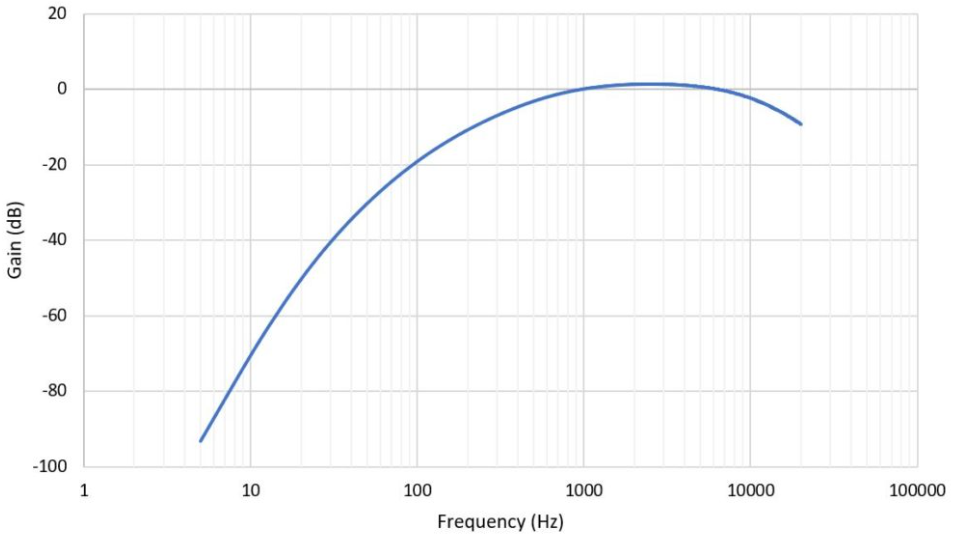
\includegraphics[width=0.6\linewidth]{figures/Propulsion/aweighting}
    \caption{A-Weighting curve \cite{aweight}}
    \label{fig:aweightcurve}
\end{figure}

The noise levels are plotted per integer multiples of the Blade Passage Frequency (BPF) up to 20 kHz,
the upper limit of the audible frequency range, in \Cref{fig:noisePlots}.
The results are plotted, and the overall SPL in dBA (OASPL) is indicated in \Cref{fig:noisePlots}, computed per each case as indicated in \Cref{eq:overalldbaspl}.
\begin{equation}
    \label{eq:overalldbaspl}
    \mathrm{OASPL} = 10\log_{10}(\int_{0}^{\infty }\frac{L(f)}{\mathrm{BPF}}\cdot df),\quad\text{with }L(f)=10^{\frac{\mathrm{SPL}(f)}{10}},\quad\text{ and }\mathrm{BPF}=\frac{B\cdot RPM}{60}
\end{equation}

\begin{figure}[H]
    \centering
    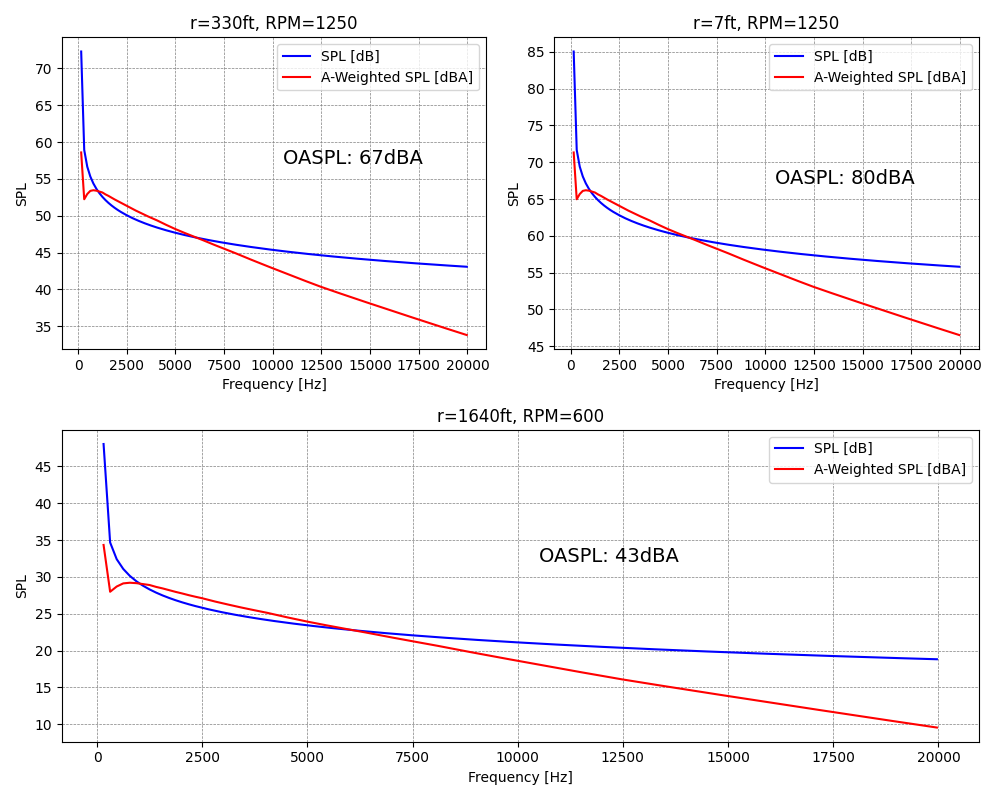
\includegraphics[width=0.85\linewidth]{figures/Propulsion/SPLSpectrum}
    \caption{SPL spectrums conforming to the noise requirements over audible frequency range, for varying distance and RPM setting.}
    \label{fig:noisePlots}
\end{figure}

The noise estimation tool was run for increasing RPM, at steps of 50 RPM, and the results of \Cref{fig:noisePlots} were the first to meet the noise requirements set to a satisfying extent.
The following values of cruise and hover RPM are therefore taken as the threshold values for the following steps of the analysis:
\begin{table}[H]
    \centering
    \begin{tabular}{ll|ll}
        \textbf{Vertical Flight Maximum RPM} & 1250 & \textbf{Cruise Flight Maximum RPM} & 600
    \end{tabular}
\end{table}
It is important to note that such values are ideally only respected during the nominal operation of the vehicle.
If, for instance, an event of emergency occurs, such values can be momentarily exceeded.

\subsection{Propeller Available Thrust Analysis}
\label{subsec:propthrustanalysis}
Now that in \Cref{subsec:propnoiseanalysis} the maximum RPM allowing to meet the noise requirements is established, it can be checked if the thrust requirement can be met within such requirements.
This is the iterative loop indicated in red in \Cref{fig:n2prop}.
Accurately estimating the thrust generated by a propeller given geometric parameters and RPM settings is no easy task, as it involves the numerical implementation of theories such as Blade Element Method (BEM) and momentum theory \cite{helicoptercourseMarilena}.
In the interest of time, such procedures are not carried out in this report, where the available thrust will, therefore, be assessed by means of empirical methods, building upon available literature on conventional aircraft propeller designs.
In wind-tunnel tests conducted by \citeauthor{nasathrustreport}~\cite{nasathrustreport} specifically, thrust curves were experimentally determined for single-rotating, six-blade propeller of \qty{3}{m} in diameter.
Such propellers were operated with Reynold’s numbers ($\mathrm{Re}$) of approximately \num{1e6}, comparable to the predicted $\mathrm{Re}$ of \num{5e6} the propellers of the \textit{Swing} will experience during operation.
The thrust coefficient, defined as in \Cref{eq:ct}, is plotted in \Cref{fig:ctvsJandRPM} against both the advance ratio $J$ and RPM, per varying $\beta$
\begin{equation}
    \label{eq:ct}
    C_T=\frac{T}{\rho n^2 D^4},\quad J=\frac{V}{nD}
\end{equation}
$n$ is the revolutions per second, and $V$ the propeller axial (freestream) velocity. As previously mentioned the blade airfoil, twist and chord distributions used in \cite{nasathrustreport} are assumed for the \textit{Swing} as well, for simplicity's sake. The blade airfoil is therefore taken to be the Clark-Y, whereas the twist and chord distributions are taken from Figure 1 of \cite{nasathrustreport}. Thanks to the assumptions above, to be reviewed in later design stages, \Cref{fig:ctvsJandRPM} can be constructed.
\begin{figure}[H]
    \centering
    \begin{subfigure}[b]{0.48\textwidth}
        \centering
        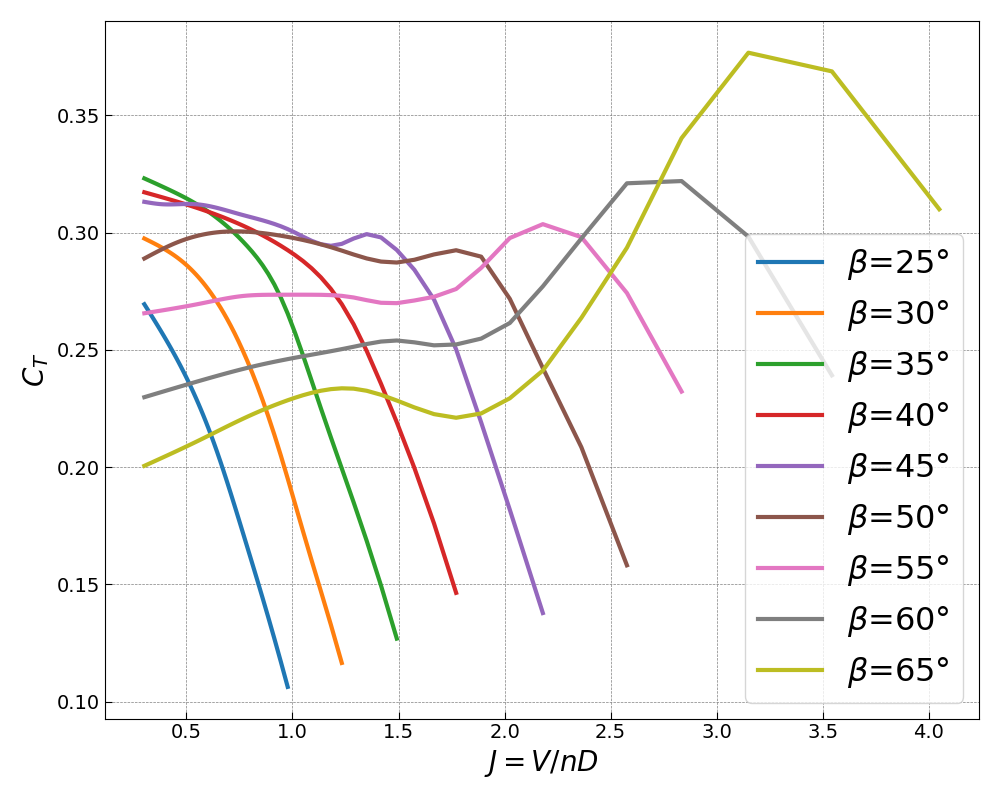
\includegraphics[width=\textwidth]{figures/Propulsion/ctvJ}
        \caption{Thrust coefficient over the advance ratio}
        \label{fig:ctvsJ}
    \end{subfigure}
    \hfill
    \begin{subfigure}[b]{0.48\textwidth}
        \centering
        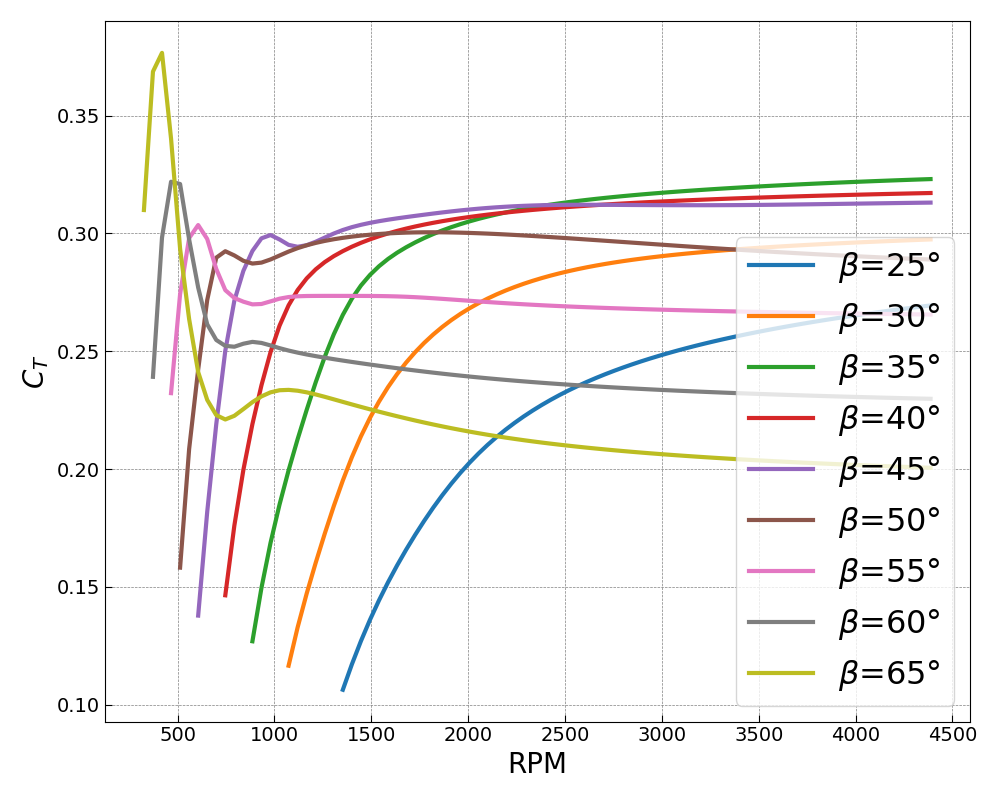
\includegraphics[width=\textwidth]{figures/Propulsion/ctvn}
        \caption{Thrust coefficient over RPM}
        \label{fig:ctvrpm}
    \end{subfigure}
    \caption{Thrust coefficient over advance ratio and RPM for a six-blade, single-rotating propeller}
    \label{fig:ctvsJandRPM}
\end{figure}
Horizontal (cruise) and vertical flight will be separately assessed in the paragraphs to follow, following from the diagrams of \Cref{fig:fbdthrust} and \Cref{fig:fbdthrust2}.

\begin{figure}[htpb]
    \centering
    \begin{minipage}[b]{0.45\textwidth}
        \centering
        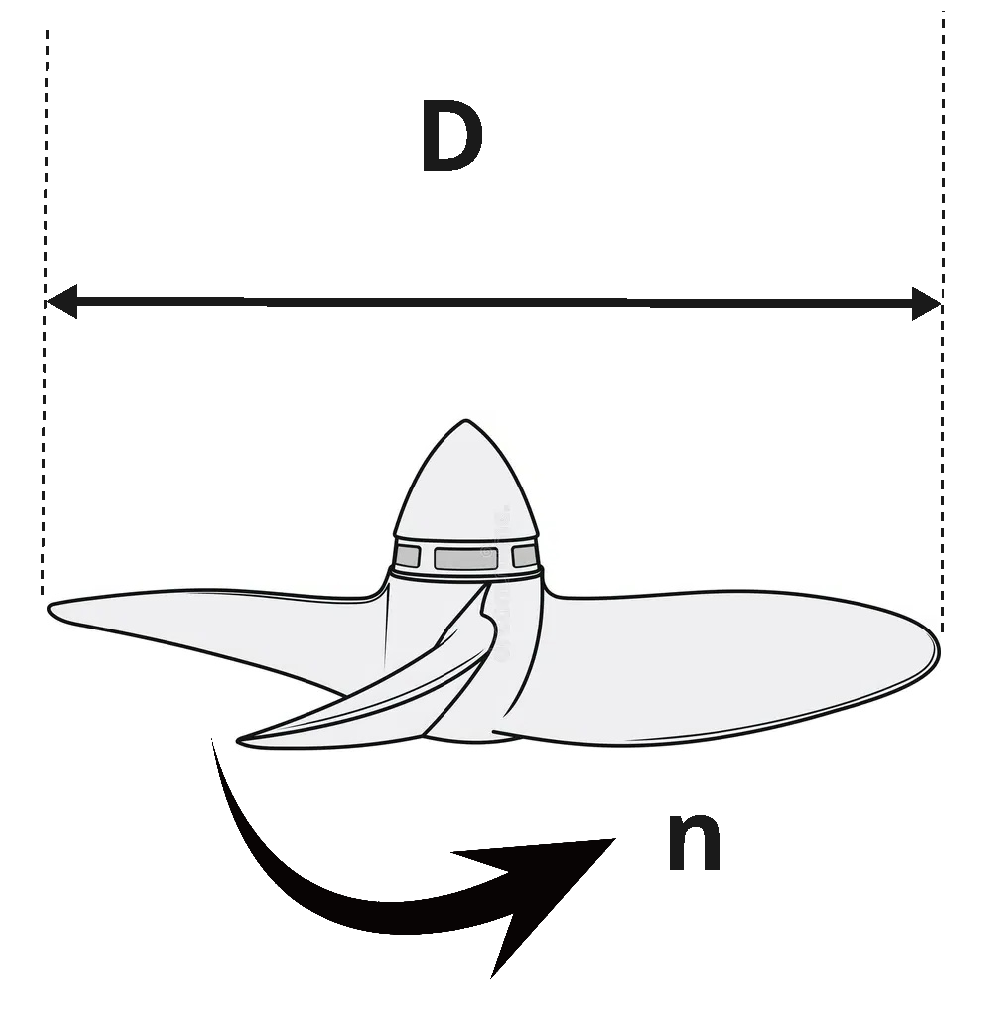
\includegraphics[width=0.9\textwidth]{figures/Propulsion/verticalprop}
        \caption{Rotor during vertical flight, $V=\qty{0}{km/h}$}
        \label{fig:fbdthrust}
    \end{minipage}
    \hspace{0.05\textwidth}
    \begin{minipage}[b]{0.45\textwidth}
        \centering
        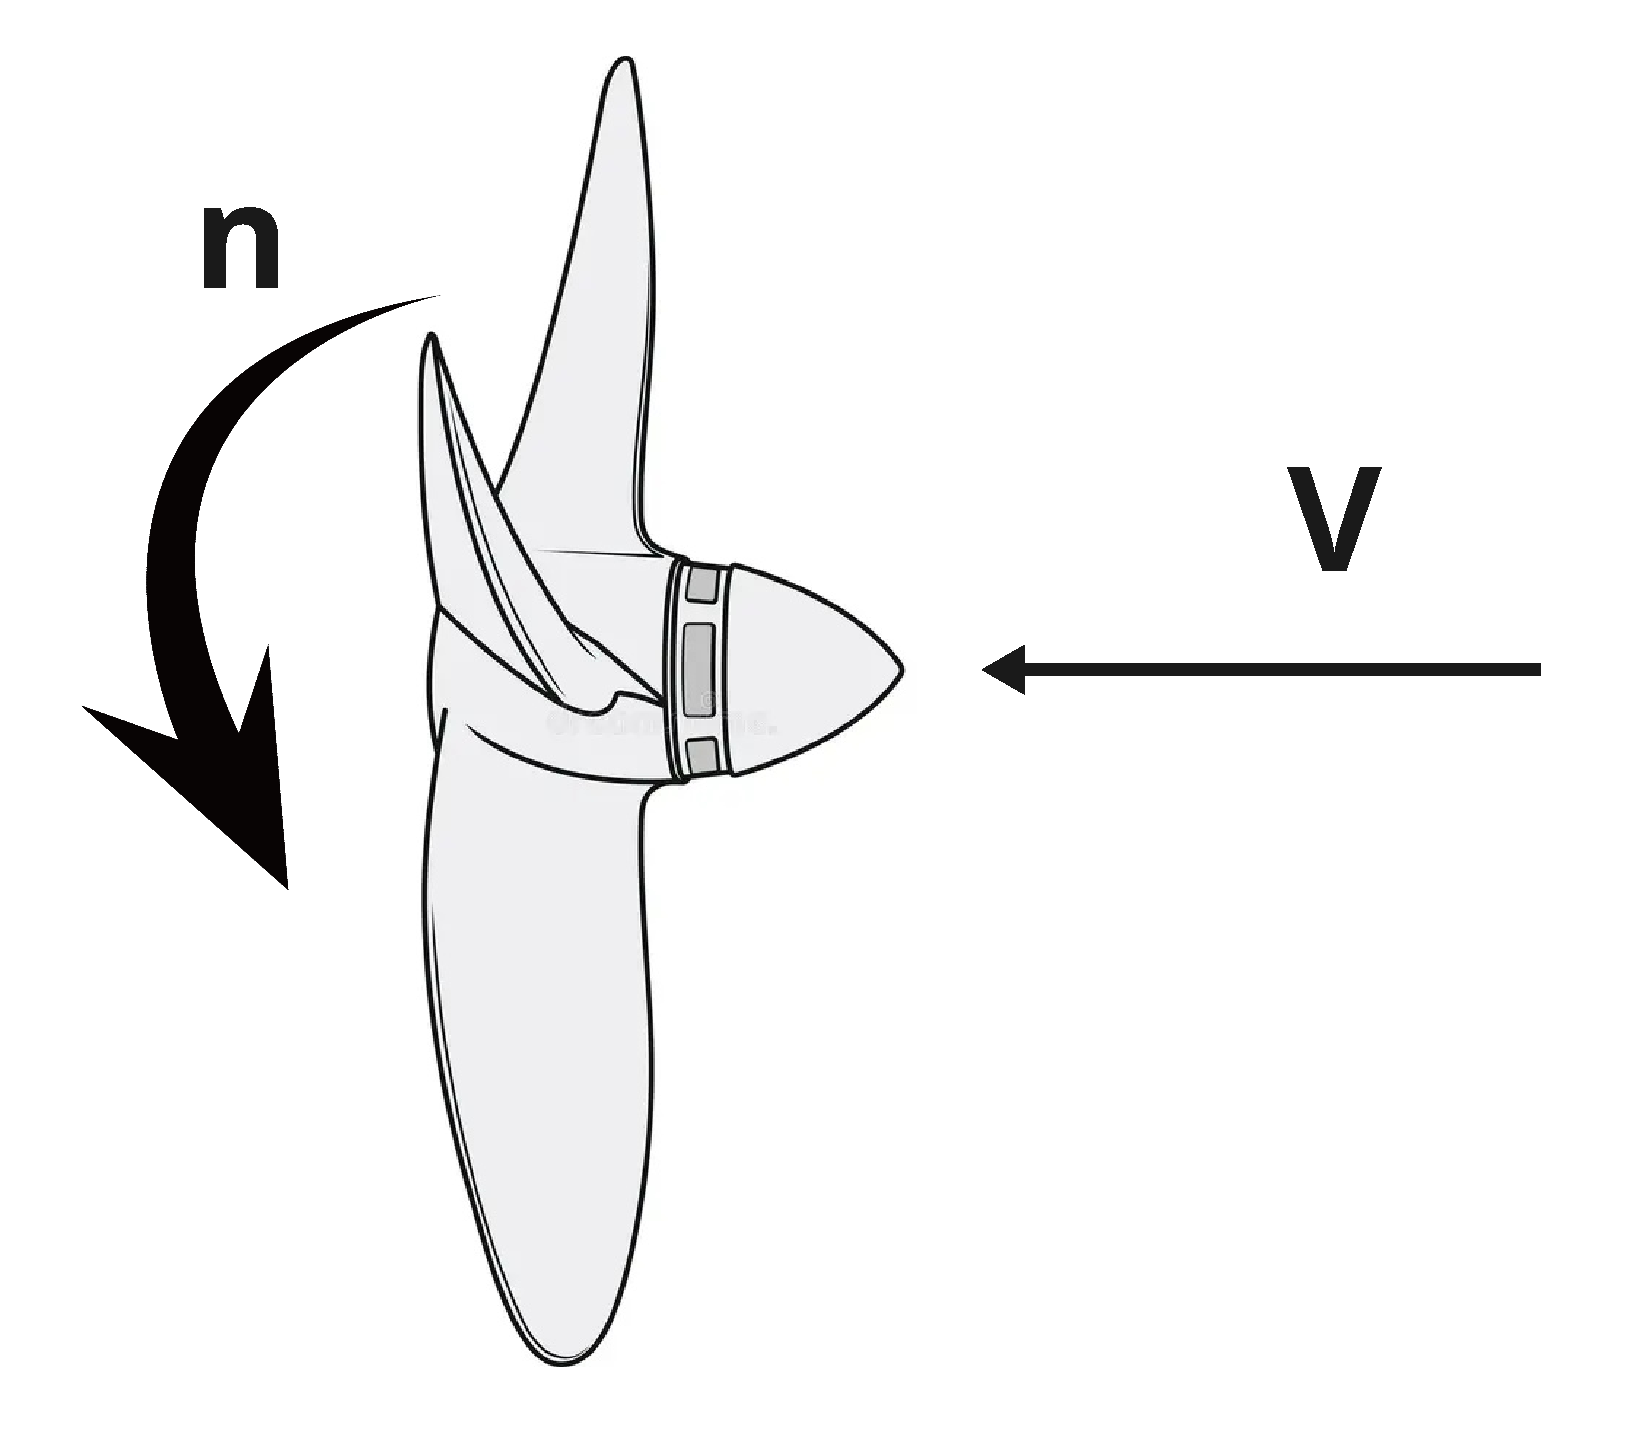
\includegraphics[width=\textwidth]{figures/Propulsion/cruiseprop}
        \caption{Propeller during horizontal flight (cruise, $V=\qty{200}{km/h}$).}
        \label{fig:fbdthrust2}
    \end{minipage}
\end{figure}

\paragraph{Available Thrust During Cruise}
Combining \Cref{fig:ctvsJ} and \Cref{fig:ctvrpm} using $V=\qty{200}{km/h}$ in $J=V/nD$, allows to plot the estimated overall thrust generated per propeller,
and under standard atmospheric conditions ($\rho=\qty{1.225}{kg/m^3}$, $Re\sim\num{1e6}$), as a function of its RPM
(throttle setting).
The result is the graph shown in \Cref{fig:thrustvsrpm}.
Here, for graphic clarity, fewer values of $\beta$ are plotted for ease of visualisation; however, the whole continuous interval $\left [ 20\degree, 65\degree \right ]$ is considered during the analysis.
\begin{figure}[H]
    \centering
    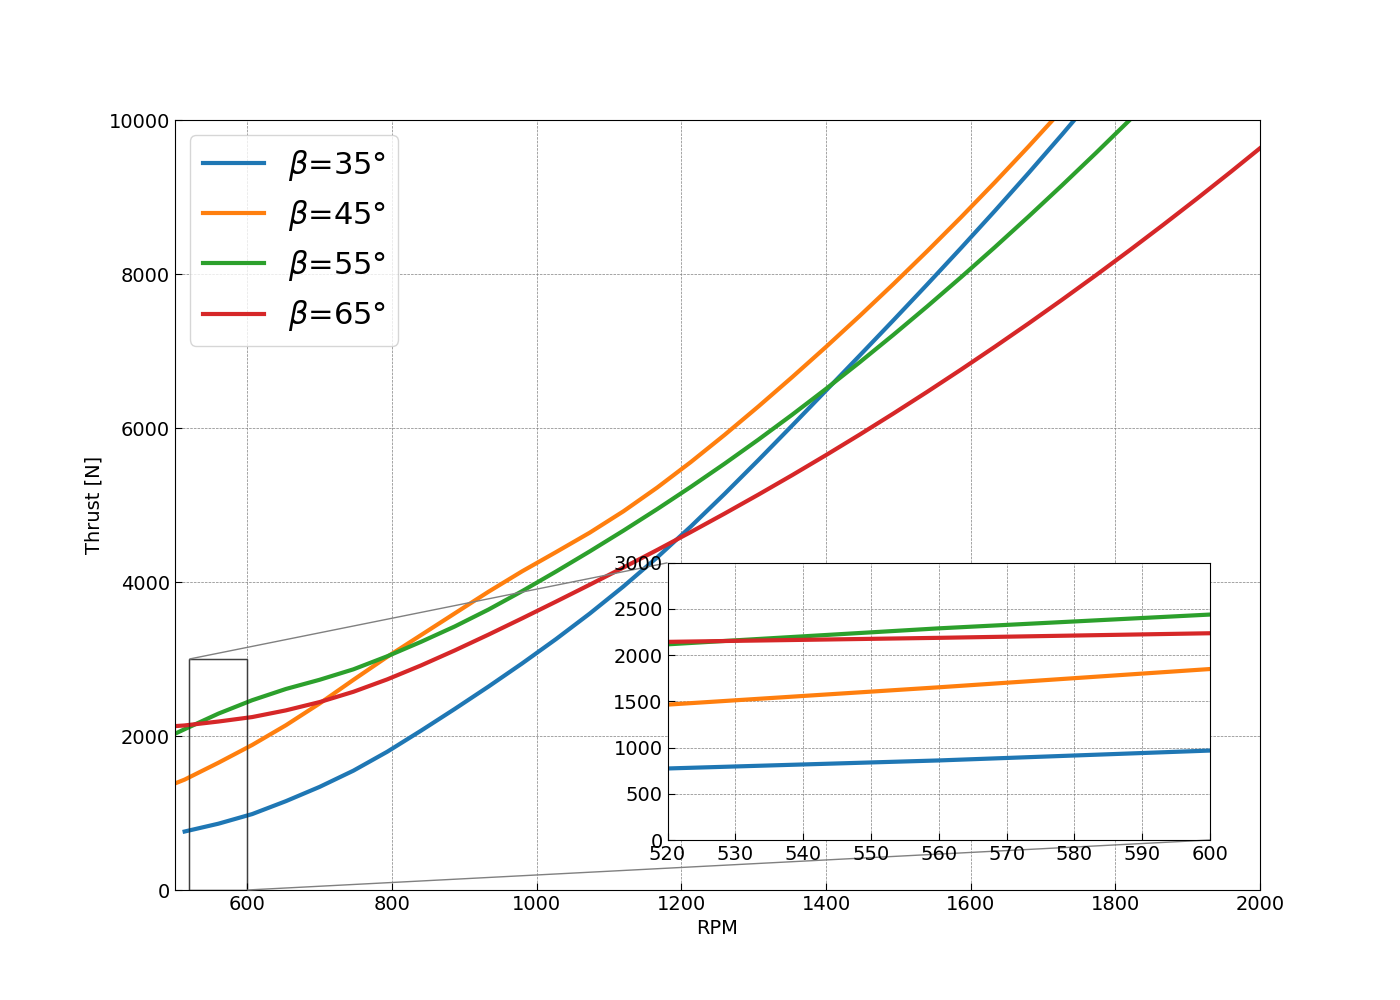
\includegraphics[width=\linewidth]{figures/Propulsion/rpmthrust}
    \caption{Thrust over RPM for a six-blade, single-rotating propeller}
    \label{fig:thrustvsrpm}
\end{figure}
Following from \Cref{fig:thrustvsrpm} is obvious that in order to meet the cruise thrust requirement of \qty{2500}{N}, translating to \qty{417}{N} per propeller during normal operations, from merely an available thrust point of view, virtually any choice of pitch angle at $0.75R$ of the blade could do the job.
It is important to note that, during the cruise, higher pitch angles are beneficial for aerodynamic efficiency as opposed to lower pitch blades \cite{proppitch}.
This is reflected in the fact that pitch angles of \qtylist[list-units=repeat]{45;55;65}{\deg} are optimal for generating thrust at lower RPM and higher values of the advance ratio (in general, higher thrust in cruise conditions).

\paragraph{Available Thrust During Vertical Flight and Hovering}
This flight condition turns out to be the most constraining, given the high thrust requirement of \qty{32000}{N}, or \qty{5333}{N} per engine (CO-3-STK03-3).
Overall phases of vertical flight, for simplicity's sake, it is assumed that the axial propeller speed be 0km/h.
This entails that $J=0$, allowing to directly read the values of $C_T$ as a function of $\beta$ from \Cref{fig:ctvsJ}. The above, through the application of \Cref{eq:ct}, are used to create the thrust curves in \Cref{fig:ctvbeta}. 
\begin{figure}[h]
    \centering
    \begin{subfigure}[b]{0.48\textwidth}
        \centering
        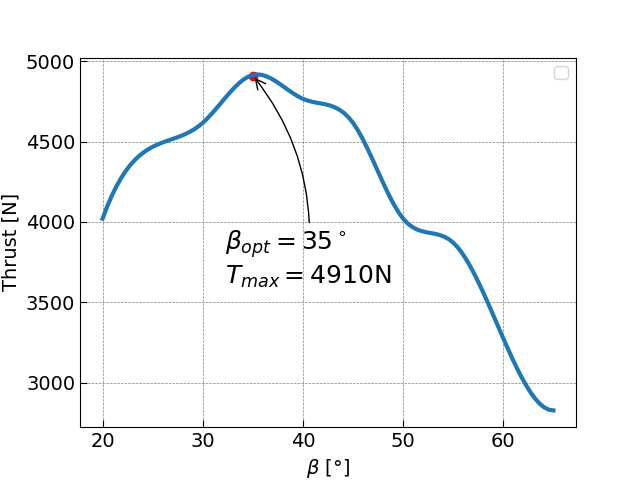
\includegraphics[width=\textwidth]{figures/Propulsion/ctvbetaUNO.png}
        \caption{Thrust as a function of pitch angle for J=0, RPM=1250. Thrust requirement can never be met}
        \label{fig:ctvb1}
    \end{subfigure}
    \hfill
    \begin{subfigure}[b]{0.48\textwidth}
        \centering
        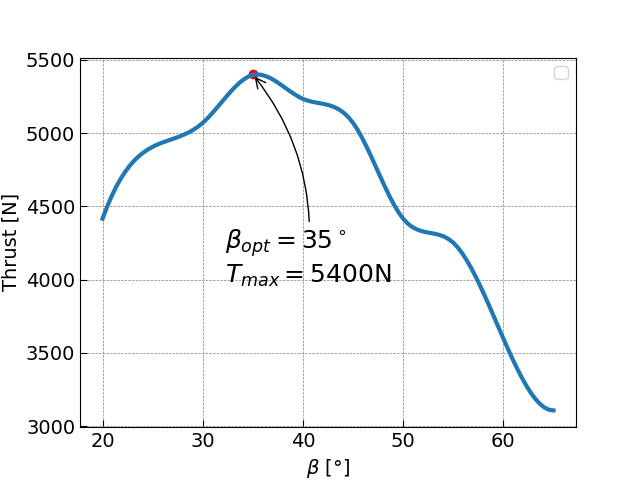
\includegraphics[width=\textwidth]{figures/Propulsion/ctvbetaDUE.png}
        \caption{Thrust as a function of pitch angle for J=0, RPM=1300. Thrust requirement is met for $\beta=35\degree$}
        \label{fig:ctvb2}
    \end{subfigure}
    \caption{Thrust curve over blade pitch angle for different RPM settings of a six-blade, single-rotating propeller}
    \label{fig:ctvbeta}
\end{figure}
As it can be seen from \Cref{fig:ctvbeta}, in order to generate the required thrust of \qty{5333}{N} per engine, the $RPM_{\max}=1250$ set in \Cref{subsec:propnoiseanalysis} is not sufficient. Indeed, in order to meet the vertical flight thrust requirement, the rotors have to rotate at 1300RPM with $\beta=35\degree$ (as shown in \Cref{fig:ctvb2}), violating the noise requirements. The exact repercussions of this result are discussed in detail in \Cref{subsec:propdesignconclusion}.

\subsection{Propeller Interference Discussion}
Due to the novel transition of the propellers, the effect of the propeller slipstream on the wing and other static surfaces should be carefully taken into account, as this will influence the previously defined performance parameters greatly.
A Stokkermans et al.
paper (2021) on the propeller slipstream influence in eVTOL configurations is of great use \cite{stokkermans2021aerodynamic}, as it dives deeper into the effects of transitioning as well, thus very valuable for this design.
The study found a strong relation of interaction effects with the geometric lay-out, as interaction effects are reduced with increasing the distance between propellers.
Moreover, during take-off and transition, the interaction effects are weak at small angle of attack (AoA), while great for larger AoA.
This is a great area of focus, due to the high AoA that is reached in the transition phase.
Furthermore, with an increasing AoA comes a greater reduction in $C_{\text{T}}$ and $C_{\text{P}}$, compared to isolated propeller configurations.
Hence, a propeller thrust loss of 30\% was even found for the rear propeller, which would result in a total power loss of up to 13\% in order to keep constant thrust by increasing the rotational speed of propellers.
However, it should be noted that the study only covered a two-propeller interaction, as well as so-called \enquote*{side-by-side} and \enquote*{one-after-another} configurations, whereas this design is a combination of the two during the transition.

Lift and drag are other parameters which greatly influence the flight performance as well; it is interesting to look at the changes due to propeller interference.
Since eVTOL configurations have propellers for vertical take-off and lading, as well as for cruise, a correct decision should be made regarding the propellers.
Whether all are the same, thus useful in both operations or if making use of redundant engines.
The last option considers having either feathered or windmilling redundant propellers; however, these are found to be less favourable for flight performance.
Since, in cruise, feathered blades can reduce lift by 25\% and increase drag up to 70\%, while for windmilling the drag can even increase by 90\% \cite{zhang2024aerodynamic}.
Although the windmilling solution could account for 50\% of the required cruise power, the redundant engines are no real viable option.
It is, however, found that the aerodynamic performance of working propellers on the wing is beneficial.
Because of the induced airflow, it seems to increase lift produced by the wing up to 8\%, while 3\% in high-lift conditions \cite{marcus2018aerodynamic}.
Therefore, it is hereby confirmed that the chosen configuration is the most beneficial for the aircraft.
Although it should be noted that the propellers were placed above the wing, and not in front of the wing, like this project’s design.
Moreover, the separation AoA is generally found to be higher, due to the propeller interference with the wing \cite{boldman1993effect}.

Because of the above-stated reasons, the propeller interaction effects can be of great help in sustaining the aircraft in the transition phase, as this phase will endure the highest AoA.

\subsection{Conclusions on Propeller Design}
\label{subsec:propdesignconclusion}
Now that the propellers have been designed in compliance with the related key requirements, conclusions can be drawn.
Given the very low thrust requirement of the \textit{Swing} during cruise, excellent noise levels can be reached while still generating more than satisfying levels of thrust, also comfortably allowing for proper handling of OEO situations and emergency manoeuvres.
During vertical flight, however, it turns out 1300 RPM are necessary to fulfil the required $T/W$ value.
Therefore, \Cref{fig:noisePlots} is generated again in \Cref{fig:newnoise}, with the new RPM value in.

\begin{figure}[htpb]
    \centering
    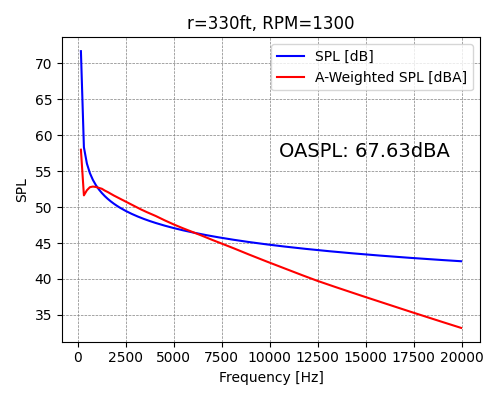
\includegraphics[width=0.5\textwidth]{figures/Propulsion/newnoise} % Adjust the width as needed
    \caption{SPL spectrum recomputed at a sample distance of 330ft, with the new RPM setting of 1300}
    \label{fig:newnoise}
\end{figure}

As it can be noted from \Cref{fig:newnoise}, the new maximum RPM setting leads to an increase in SPL of 0.63dBA,
meaning a roughly 12\% louder aircraft, thus slightly violating the noise requirements.
However, it is important to note that such high-thrust (and therefore high-RPMs, ultimately leading to high SPL) flight conditions will rarely be met during normal operations.
Lastly, a blade pitch angle at $0.75R$ ($\beta$) of $35\degree$ is chosen, offering optimal performances during vertical flight and transition, and slightly suboptimal performances during cruise (optimal cruise pitch would be around $55\degree$). Achieving optimal performance during cruise would, therefore, require the implementation of a variable propeller pitch system, the complexity and cost of which was considered to not outweigh its -not so substantial- advantages.

\section{Motor Selection}
\label{sec:engineschoice}
% max engine thrustr is hard to establish as youd need precise power curve of engine WITH mounted prop... we can give an estimate
Since the propellers have now been properly sized, as well as its performance parameters, the trade-off on the end of the motor selection can be performed.
In the interest of cost, time and vehicle reliability, it was decided to opt for using OTS electric motors, specifically designed and optimised for eVTOLs.
An extensive literature study was performed to identify state-of-the-art, certified electric engines suitable for UAM applications.
Bearing in mind the total power requirement of $\qty{343}{kW}/6=\qty{56}{kW}$ per engine from \Cref{subsec:transition},
only the motors capable of delivering at least 56 kW of continuous maximum power\footnote{Power which can be continuously delivered to the propeller for more than 60 seconds.} ($P_{\max}$) are presented in \Cref{tab:motor_trade-off}.

\begin{table}[H]
    \caption{Tabulated results of motors literature study}
    \label{tab:motor_trade-off}
    \resizebox{\textwidth}{!}{%
        \begin{tabular}{
            @{}
            l|
            S[table-format=3.0]
            S[table-format=3.0]
            S[table-format=5.0]
            l
            S[table-format=3.1]
            S[table-format=1.1, table-auto-round]
            S[table-format=4.0]
            c
            @{}
        }
            \toprule
            & \textbf{$P_{\max}$ {[}kW{]}} & \textbf{$T_{\text{peak}}$ {[}Nm{]}} & \multicolumn{2}{c}{\textbf{$RPM_{\max}$ (@$P_{\text{peak}}$)}} & \textbf{Mass {[}kg{]}} & \textbf{$P/W$ {[}kW/kg{]}} & \textbf{$P_{\text{peak}_{\text{tot}}}$ {[}kW{]}} & \textbf{$D\times L$ {[}mm{]}} \\ \midrule
            Emrax 208       & 56                                 & 90                                  & 6000 & (86)                                        & 10.3                   & 5.44                           & 336                                              & \numproduct{208x85}                \\
            Emrax 228       & 75                                 & 130                                 & 6500 & (124)                                       & 13.5                   & 5.56                           & 450                                              & \numproduct{228x86}                \\
            Evo Motor AF340 & 282                                & 780                                 & 5000 & (660)                                       & 122                    & 2.31                           & 1692                                             & \numproduct{380x333}               \\
            MagniX Magni350 & 320                                & {-}                                   & 2300 & (350)                                       & 128                    & 2.5                            & 1920                                             & \numproduct{675x550}               \\
            Remy HVH250HT   & 100                                & 440                                 & 10600 & (150)                                      & 43                     & 2.33                           & 600                                              & \numproduct{242x180}               \\
            Rotex REB 90    & 30                                 & {-}                                   & 2800 & (80)                                        & 23                     & 1.3                            & 180                                              & \numproduct{270x212}               \\
            Yasa 750R       & 70                                 & 400                                 & 3250 & (200)                                       & 37                     & 1.9                            & 420                                              & \numproduct{368x98}  \\
            \bottomrule
        \end{tabular}% 
    }
\end{table}
With $T_{\text{peak}}$ being the maximum torque that can be exerted by the engine. $P_{\text{peak}}$, as opposed to $P_{\max}$, is the power that can be delivered by the engine only in short bursts of a couple of seconds.
$D$ is the motor diameter, $L$ the motor length.
Based on \Cref{tab:motor_trade-off}, a quick trade-off is set up and performed in \Cref{tab:motortradeoff}, where each criterion is given an equal weight of 25\% (column widths are not to scale).
Scores are given on a scale from 1 to 5 according to \Cref{tab:motor_trade-off}, rounding \Cref{eq:scoring} to the nearest integer.
\begin{equation}
    \label{eq:scoring}
    \text{rescaled value} = 1 + \left( \frac{\text{value} - \min \text{value}}{\max \text{value} - \min \text{value}} \right) \times (5 - 1)
\end{equation}


\begin{table}[H]
    \centering
    \caption{Motor selection trade-off summary table}
    \label{tab:motortradeoff}
    \sisetup{table-format=1}
    \begin{tabular}{l||S|S|S|S||S[table-format=1.1, table-auto-round]}
        \toprule
        \textbf{Motor} & \textbf{Mass}          & \textbf{P/W}           & \textbf{D}             & \textbf{L} & \bfemph{Score} \\\bottomrule
        Emrax 228                            & \cellcolor{green!50}5  & \cellcolor{green!50}5  & \cellcolor{green!50}5  & \cellcolor{green!50}5 & \cellcolor{green!50}5 \\
        Evo Motor AF340                      & \cellcolor{red!50}1    & \cellcolor{red!50}1    & \cellcolor{red!50}1    & \cellcolor{yellow!50}4 & \cellcolor{yellow!25!green!25}2.25 \\
        MagniX Magni350                      & \cellcolor{red!50}1    & \cellcolor{orange!50}2 & \cellcolor{red!50}1    & \cellcolor{red!50}1 & \cellcolor{red!50!yellow!50}1.25 \\
        Remy HVH250HT                        & \cellcolor{yellow!50}4 & \cellcolor{red!50}1    & \cellcolor{yellow!50}4 & \cellcolor{yellow!50}5 & \cellcolor{yellow!50}3.5 \\
        Yasa 750R
        & \cellcolor{yellow!50}4 & \cellcolor{red!50}1    & \cellcolor{yellow!50}4 & \cellcolor{green!50}5 & \cellcolor{yellow!50}3.5 \\
        \toprule
    \end{tabular}
\end{table}

It is clear that the Emrax 228 wins this trade-off.
Given an expected maximum RPM of 1300 and a maximum torque experienced, during transition, of $T_{\max}=525.2\cdot \mathrm{PHP}/\mathrm{RPM}=\qty{70}{Nm}$ (given the shaft horsepower per engine $\mathrm{PHP}$, and rotor RPM), the Emrax 228 is selected as the engine to be mounted on the \textit{Swing}.


\section{Verification and Validation (V\&V)}
\label{sec:propulsionVandV}
In this section, the computational models used in \Cref{subsec:propnoiseanalysis} and \Cref{subsec:propthrustanalysis} to size the propulsion subsystem will be verified and validated.
For verification, the models are to be checked for correctness of implementation and coherence with the underlying theory.
During validation, the results provided by the models are checked against known real-life results, allowing the model to be deemed reliable \cite{dsePMSESlides1}.

\subsection{Noise Model V\&V}
\label{subsec:noisevev}
\paragraph{Verification}As previously explained, the noise model derives from the direct implementation of the procedure outlined in \cite{noiseNASA}.
Unit tests were performed on individual code functions to make sure plotting and basic calculations were working in order and according to theory.
Moreover, results and plot trends comparable to those found in \cite{noiseNASA} are obtained in \Cref{subsec:propnoiseanalysis}, therefore allowing to confidently state the model is verified - as its results are in full accordance with the theoretical framework it is based on.
\paragraph{Validation}With respect to model validation, it was chosen to run the tool with parameters taken from the Joby aircraft (listed in \Cref{tab:jobyparams}), for which an in-depth noise analysis was performed \cite{nasaxjoby2022acoustic}, allowing it to compare its results against those outputted by the model of~\Cref{subsec:propnoiseanalysis}.
Running the tool with the parameters indicated below for various distances (in ft) at which the
noise is to be calculated, leading to the plots of \Cref{fig:jobynoiseours}.
\begin{table}[H]
    \centering
    \caption{Joby parameters used for noise model validation}
    \label{tab:jobyparams}
    \begin{tabular}{S[table-format=1]S[table-format=1]S[table-format=3]S[table-format=3]}
        \toprule
        \textbf{Rotor diameter [ft]} & \textbf{Blade count per rotor [-]} & \textbf{Hovering RPM} & \textbf{Hovering Power [kW]} \\ \midrule
        6                            & 5                                  & 800                   & 411 \\
        \bottomrule
    \end{tabular}
\end{table}

\begin{figure}[h]
    \centering
    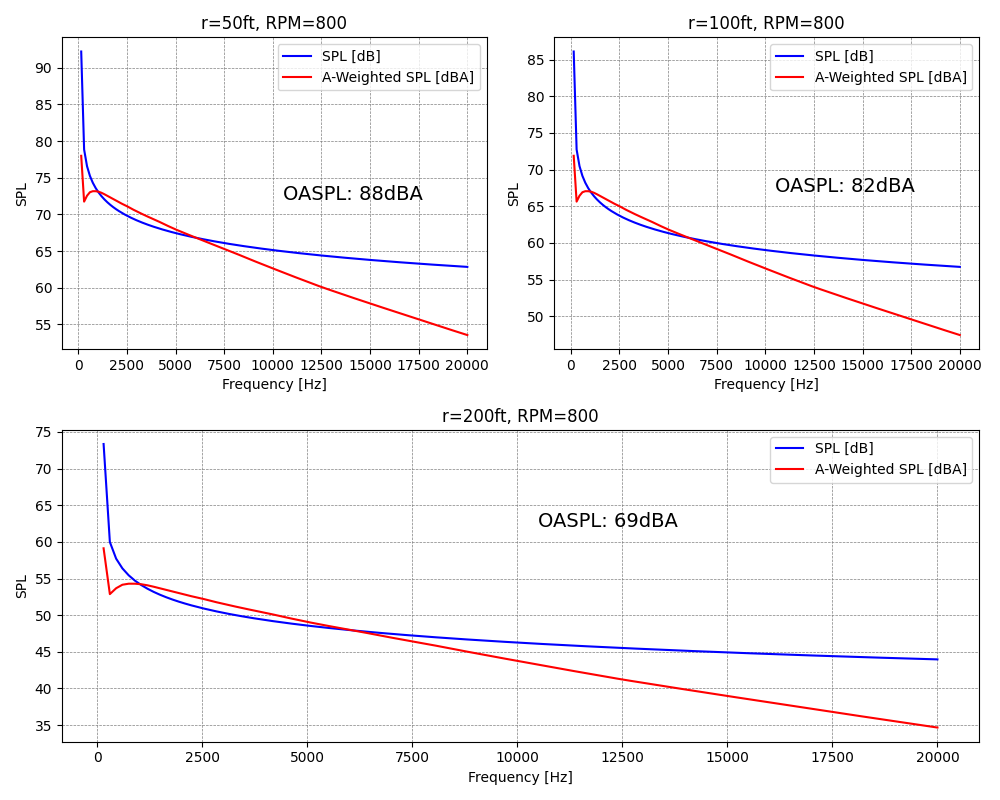
\includegraphics[width=0.9\linewidth]{figures/Propulsion/jobynoiseours}
    \caption{Output of the noise model running on Joby parameters}
    \label{fig:jobynoiseours}
\end{figure}
From \Cref{fig:jobynoisetakeoff} the actual vehicle noise in dBA can be determined, at vertical distances of \qtylist{50;100;200}{ft}.
Putting together the information from \Cref{fig:jobynoisetakeoff,fig:jobynoiseours}, \Cref{tab:noisevalidation} can be constructed, summarising the results of this validation procedure.

\begin{table}[H]
    \centering
    \caption{Tabulated results of the noise model validation procedure}
    \label{tab:noisevalidation}
    \begin{tabular}{S[table-format=3]|S[table-format=2]S[table-format=2]}
        \toprule
        \textbf{Vertical Distance [\unit{ft}]} & \textbf{Actual Noise [\unit{dBA}]} & \textbf{Simulated Noise [\unit{dBA}]} \\ \midrule
        50 & 85 & 88 \\
        100 & 75 & 82 \\
        200 & 62 & 69 \\
        \bottomrule
    \end{tabular}
\end{table}

From \Cref{tab:noisevalidation} it can be observed that the model of \Cref{subsec:propnoiseanalysis} consistently overestimates the OASPL generated.
This result is considered beneficial, as it suggests that there is room for further improving the generated OASPL of the \textit{Swing} by aerodynamic optimisations of the vehicle surfaces (both lifting and non-lifting).

\begin{figure}[htpb]
    \centering
    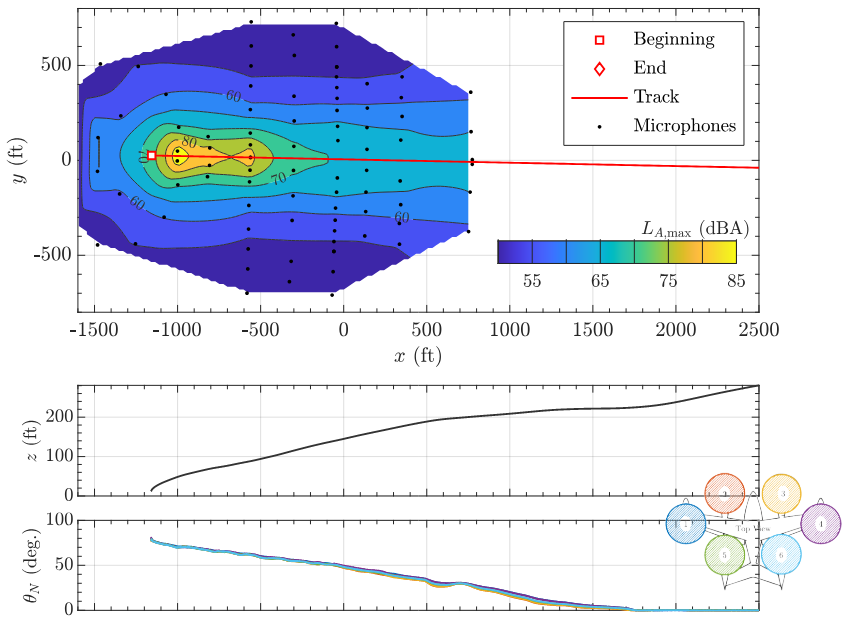
\includegraphics[width=0.8\linewidth]{figures/Propulsion/Joby-noise-takeoff}
    \caption{Noise analysis empirically performed on Joby}
    \label{fig:jobynoisetakeoff}
\end{figure}


\subsection{Thrust Model V\&V}
\label{subsec:thrustvev}
\paragraph{Verification}As for the noise model, the thrust model outlined in \Cref{subsec:propthrustanalysis} is considered to be verified by appropriate unit tests and accordance; comparing \Cref{fig:ctvsJ} against the corresponding graphs in \cite{nasathrustreport} allows proving the model was implemented correctly.
\paragraph{Validation}To instead validate the model, a sensitivity analysis will be performed.
As it can be seen from \Cref{fig:n2prop}, rotor diameter ($D$), blade count ($B$) and RPM are inputs to the thrust model.
From this, \Cref{tab:sensitivitythrust} can be constructed.
\begin{table}[H]
    \centering
    \begin{tabular}{l|ccc}
        \toprule
        \textbf{Variable Change} & \textbf{Expected Output} & \textbf{Model Output} & \textbf{Pass/Fail} \\
        \midrule
        $B \downarrow$           & $T \downarrow$           & $T \downarrow$        & Pass               \\
        $D \uparrow$             & $T \uparrow$             & $T \uparrow$          & Pass               \\
        $D \downarrow$           & $T \downarrow$           & $T \downarrow$        & Pass               \\
        $RPM \uparrow$           & $T \uparrow$             & $T \uparrow$          & Pass               \\
        $RPM \downarrow$         & $T \downarrow$           & $T \downarrow$        & Pass               \\
        \bottomrule
    \end{tabular}
    \caption{Variable changes and their effects on thrust output}
    \label{tab:sensitivitythrust}
\end{table}
Following the results of \Cref{tab:sensitivitythrust}, the thrust model is said to be validated.



